\documentclass[aspectratio=169,11pt]{beamer}
% Shared Beamer setup for Ms Economía PEG, Problem Set 1, Team 3.
\usepackage[T1]{fontenc}
\usepackage[utf8]{inputenc}
\usepackage[spanish,es-noshorthands]{babel}
\usepackage{booktabs}
\usepackage{graphicx}
\usepackage{amsmath,amssymb}
\usepackage{tabularx}
\usepackage{xcolor}
\usepackage{tikz}
\usepackage{hyperref}

\graphicspath{{../02_outputs/figures/}{img/}{./}}
\newcommand{\nsample}{14,761}
\newcommand{\ntrain}{10,260}
\newcommand{\nvalid}{4,501}
\newcommand{\sharefemale}{47.3}
\newcommand{\medianincome}{992,745}
\newcommand{\meanincome}{1,617,237}
\newcommand{\medianhours}{48}
\newcommand{\meanage}{38.9}
\newcommand{\peakuncond}{40.6}
\newcommand{\peakuncondlo}{40.1}
\newcommand{\peakuncondhi}{41.2}
\newcommand{\peakcond}{43.6}
\newcommand{\peakcondlo}{42.8}
\newcommand{\peakcondhi}{44.5}
\newcommand{\rtwoageu}{0.050}
\newcommand{\rtwoagec}{0.226}
\newcommand{\gapuncond}{-21.2}
\newcommand{\gaphc}{-27.2}
\newcommand{\gappref}{-19.6}
\newcommand{\gapjob}{-18.9}
\newcommand{\gapcoef}{-0.218}
\newcommand{\gapse}{0.012}
\newcommand{\gapseboot}{0.012}
\newcommand{\fwlcoef}{-0.218}
\newcommand{\peakmen}{50.5}
\newcommand{\peakmenlo}{49.1}
\newcommand{\peakmenhi}{52.3}
\newcommand{\peakwomen}{45.6}
\newcommand{\peakwomenlo}{44.4}
\newcommand{\peakwomenhi}{47.0}
\newcommand{\bestmodel}{P6: Flexible age, education, and hours}
\newcommand{\bestshort}{P6: polinomio flexible}
\newcommand{\gapuncondabs}{21.2}
\newcommand{\gaphcabs}{27.2}
\newcommand{\gapprefabs}{19.6}
\newcommand{\bestvalid}{0.6160}
\newcommand{\bestloocv}{0.5825}
\newcommand{\besttrain}{0.5797}
\newcommand{\topvar}{Socioeconomic stratum}
\newcommand{\topdelta}{0.1185}


\definecolor{navy}{HTML}{1B365D}
\definecolor{accent}{HTML}{B85C38}
\definecolor{slate}{HTML}{5B6B73}
\definecolor{gold}{HTML}{C4A35A}
\definecolor{ice}{HTML}{F4F6F8}

\setbeamercolor{structure}{fg=navy}
\setbeamercolor{frametitle}{fg=navy,bg=white}
\setbeamercolor{title}{fg=navy}
\setbeamercolor{subtitle}{fg=slate}
\setbeamercolor{author}{fg=slate}
\setbeamercolor{institute}{fg=slate}
\setbeamercolor{date}{fg=slate}
\setbeamercolor{item}{fg=accent}
\setbeamercolor{footline}{fg=slate}
\setbeamercolor{normal text}{fg=navy}

\setbeamertemplate{navigation symbols}{}
\setbeamertemplate{itemize items}[circle]
\setbeamerfont{frametitle}{series=\bfseries,size=\large}
\setbeamerfont{title}{series=\bfseries,size=\LARGE}

% Escudo Uniandes: portada y esquina superior derecha de cada diapositiva.
\newcommand{\uniandeslogo}[1][0.92cm]{
\includegraphics[height=#1]{logo_uniandes.png}}

\setbeamertemplate{frametitle}{%
  \nointerlineskip
  \vspace{0.18cm}%
  \leavevmode
  \hbox to \textwidth{%
    \begin{minipage}[c]{0.88\textwidth}
      \raggedright
      \usebeamerfont{frametitle}\usebeamercolor[fg]{frametitle}\insertframetitle
    \end{minipage}%
    \hfil
    \raisebox{-0.12cm}{\uniandeslogo[0.72cm]}%
  }%
  \vspace{0.12cm}%
}

\setbeamertemplate{title page}{%
  \vbox{}
  \vspace{0.15cm}
  \begin{flushright}
    \uniandeslogo[1.15cm]
    \hspace{0.08cm}
  \end{flushright}
  \vspace{0.55cm}
  \begin{center}
    {\usebeamerfont{title}\usebeamercolor[fg]{title}\inserttitle\par}
    \vspace{0.45em}
    {\usebeamerfont{subtitle}\usebeamercolor[fg]{subtitle}\insertsubtitle\par}
    \vspace{1.15em}
    {\usebeamerfont{author}\insertauthor\par}
    \vspace{0.55em}
    {\usebeamerfont{institute}\insertinstitute\par}
    \vspace{0.85em}
    {\usebeamerfont{date}\insertdate\par}
  \end{center}
}

\setbeamertemplate{footline}{
  \leavevmode%
  \hbox{%
    \begin{beamercolorbox}[wd=.55\paperwidth,ht=2.4ex,dp=1.2ex,leftskip=1em]{footline}
      \tiny Grupo 3 $\cdot$ Ms Economía PEG $\cdot$ Universidad de los Andes
    \end{beamercolorbox}%
    \begin{beamercolorbox}[wd=.45\paperwidth,ht=2.4ex,dp=1.2ex,rightskip=1em,right]{footline}
      \tiny \insertframenumber/\inserttotalframenumber
    \end{beamercolorbox}}%
  \vskip0pt%
}

\newcommand{\statblock}[3]{%
  \begin{tikzpicture}
    \node[fill=ice, inner sep=10pt, text width=0.42\textwidth, align=center] {
      {\fontsize{20}{24}\selectfont\bfseries\color{navy} #1}\\[4pt]
      {\small\color{slate} #2}\\[2pt]
      {\scriptsize\color{accent} #3}
    };
  \end{tikzpicture}%
}

\newcommand{\source}[1]{\vfill{\scriptsize\color{slate} #1}}


\title{Predicci\'on de ingreso laboral}
\subtitle{Problem Set 1 $\cdot$ Secci\'on 3}
\author{Juli\'an Herrera \and Andr\'es Silva \and Valentina Vera}
\institute{Ms Econom\'ia PEG $\cdot$ Big Data and Machine Learning para Econom\'ia Aplicada\\ Universidad de los Andes}
\date{2026-20 $\cdot$ Grupo 3}

\begin{document}

\begin{frame}[plain]
  \titlepage
\end{frame}

\begin{frame}{Result overview}

\vspace{0.5em}

\begin{center}
\begin{tabular}{@{}c@{\hspace{1.2cm}}c@{}}

% -------- CARD 1 --------
\fcolorbox{black!12}{black!3}{
  \begin{minipage}[c][3.15cm][c]{0.38\textwidth}
    \centering

    {\usebeamercolor[fg]{structure}
    \fontsize{27}{30}\selectfont
    \bestvalid\par}

    \vspace{0.35em}

    {\large RMSE de validaci\'on\par}

    \vspace{0.45em}

    {\small
    \textbf{S2: Preferred gender gap}
    \par}
  \end{minipage}
}

&

% -------- CARD 2 --------
\fcolorbox{black!12}{black!3}{
  \begin{minipage}[c][3.15cm][c]{0.38\textwidth}
    \centering

    {\usebeamercolor[fg]{structure}
    \Large\textbf{Stratum}\par}

    \vspace{0.35em}

    {\large predictor m\'as importante\par}

    \vspace{0.45em}

    {\small
    $\Delta$RMSE = \textbf{\topdelta}
    al permutar
    \par}
  \end{minipage}
}

\end{tabular}
\end{center}

\vspace{1.0em}

\begin{center}
\begin{minipage}{0.88\textwidth}

\textbf{Muestra de entrenamiento:}
chunks 1--7 ($N=\ntrain$)

\vspace{0.25em}

\textbf{Muestra de validaci\'on:}
chunks 8--10 ($N=\nvalid$)

\vspace{0.25em}

\textbf{LOOCV del modelo seleccionado:}
\bestloocv

\end{minipage}
\end{center}

\vfill

\source{P\'erdida: RMSE en $\log$ ingreso laboral mensual. LOOCV v\'ia f\'ormula de leverage.}

\end{frame}

\begin{frame}{RMSE de validaci\'on}
  \begin{center}
    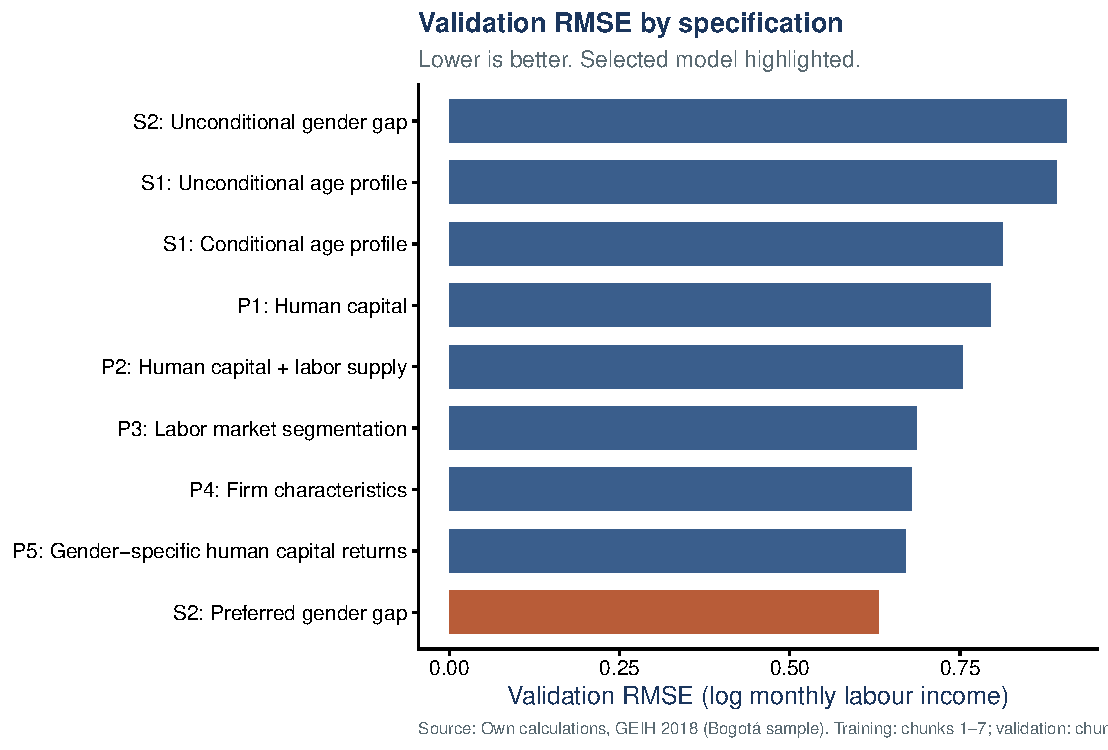
\includegraphics[width=0.82\textwidth]{fig_validation_rmse.pdf}
  \end{center}
\end{frame}

\begin{frame}{Todas las especificaciones}
  \begin{center}
    \scriptsize
    \resizebox{0.98\textwidth}{!}{\begin{tabular}{llccc}
\toprule
Model & Origin & Training RMSE & Validation RMSE & Training R$^2$ \\
\midrule
S2: Preferred gender gap & Section 2 & 0.6028 & 0.6306 & 0.539 \\
P5: Gender-specific human capital returns & Additional & 0.6396 & 0.6701 & 0.481 \\
P4: Firm characteristics & Additional & 0.6486 & 0.6795 & 0.467 \\
P3: Labor market segmentation & Additional & 0.6599 & 0.6861 & 0.448 \\
P2: Human capital + labor supply & Additional & 0.7275 & 0.7541 & 0.329 \\
P1: Human capital & Additional & 0.7812 & 0.7942 & 0.226 \\
S1: Conditional age profile & Section 1 & 0.7781 & 0.8118 & 0.232 \\
S1: Unconditional age profile & Section 1 & 0.8656 & 0.8919 & 0.050 \\
S2: Unconditional gender gap & Section 2 & 0.8804 & 0.9066 & 0.017 \\
\bottomrule
\end{tabular}
}
  \end{center}

  \source{El $R^2$ de entrenamiento no elige el modelo. El criterio de selecci\'on es RMSE de validaci\'on.}
\end{frame}

\begin{frame}{LOOCV contra validaci\'on}
  \begin{center}
    \footnotesize
    \begin{tabular}{lccc}
\toprule
Model & Training RMSE & LOOCV RMSE & Validation RMSE \\
\midrule
S2: Preferred gender gap & 0.6028 & 0.6044 & 0.6306 \\
\bottomrule
\end{tabular}

  \end{center}

  \vspace{0.6em}
  \begin{itemize}
    \item LOOCV calcula el error dejando una observaci\'on fuera cada vez.
    \item Para OLS usamos $\tilde{\varepsilon}_i=\hat{\varepsilon}_i/(1-h_{ii})$, equivalente a reestimar $n$ veces.
    \item LOOCV y validaci\'on son relativamente cercanos, lo que sugiere estabilidad razonable del desempe\~no predictivo.
  \end{itemize}
\end{frame}

\begin{frame}{Importancia: permutaci\'on en validaci\'on}
  \begin{center}
    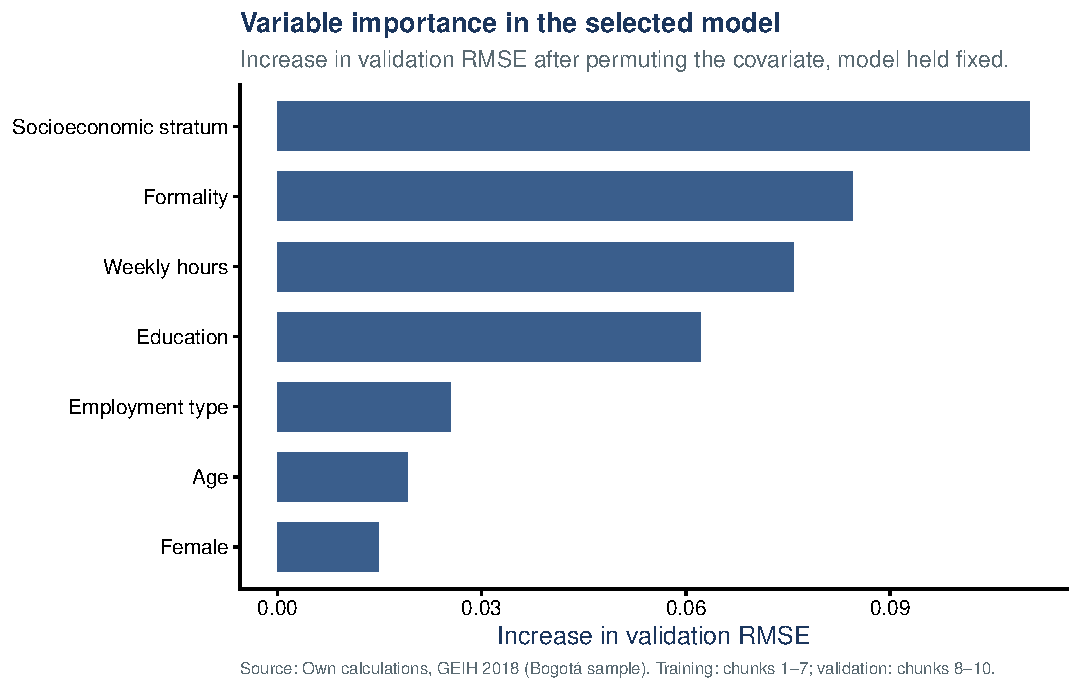
\includegraphics[width=0.92\textwidth]{fig_variable_importance.pdf}
  \end{center}

  \source{La importancia se mide como el aumento en RMSE al permutar cada covariable, manteniendo fijo el modelo.}
\end{frame}

\begin{frame}{C\'omo predice el modelo en funci\'on de \topvar}
  \begin{center}
    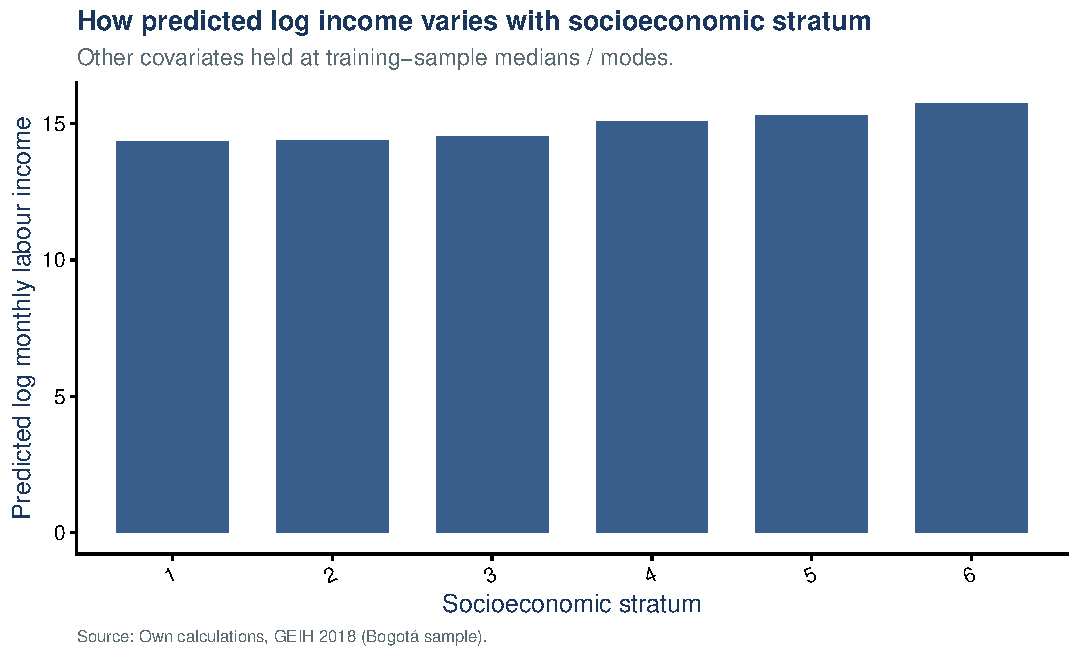
\includegraphics[width=0.92\textwidth]{fig_prediction_partial_dependence.pdf}
  \end{center}

  \source{Las dem\'as covariables se mantienen en valores t\'ipicos de entrenamiento. No es una interpretaci\'on causal.}
\end{frame}

\begin{frame}{D\'onde se rompe la predicci\'on}
  \begin{center}
    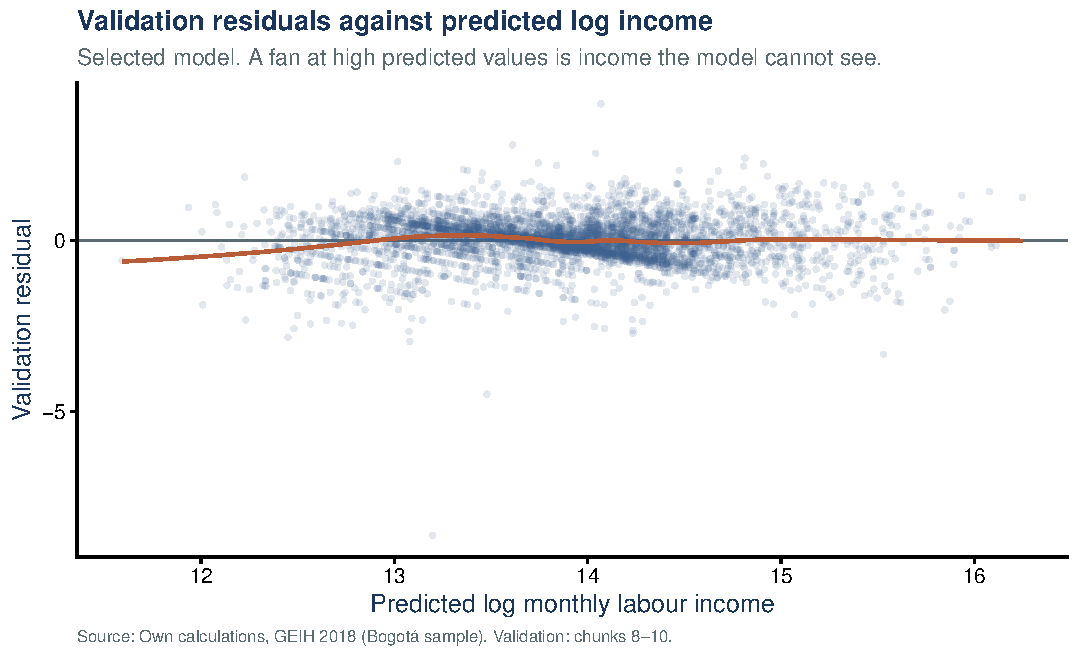
\includegraphics[width=0.92\textwidth]{fig_validation_residuals.pdf}
  \end{center}
\end{frame}

\begin{frame}{Lectura para la autoridad tributaria}
  \begin{itemize}
    \item El mejor modelo es \textbf{\bestshort}. Ninguna especificaci\'on se escoge por relato: gana la que minimiza el RMSE de validaci\'on.
    \item \topvar\ es la variable cuya permutaci\'on deteriora m\'as la predicci\'on. Esto indica importancia predictiva, no causalidad.
    \item Los residuales muestran d\'onde el modelo falla. Para una autoridad tributaria, el modelo puede ayudar a priorizar casos, pero no debe automatizar auditor\'ias.
  \end{itemize}

  \vspace{0.4em}
  \begin{block}{Takeaway}
    \bestshort\ minimiza el RMSE de validaci\'on (\bestvalid). LOOCV es consistente con este resultado (\bestloocv). El predictor m\'as importante es \topvar.
  \end{block}
\end{frame}

\end{document}